\begin{center}
	\vspace{0.5cm}{\parbox{16cm}{\small{\centering{\textbf{Аннотация}\\
					\hspace{0.6cm} В этом отчёте изложены результаты выполнения лабораторной работы «Инфракрасная спектроскопия поглощения.
					Колебательно-вращательные спектры
					двухатомных молекул». В данной работе исследуется вращательная структура основной
					колебательно-вращательной полосы поглощения молекулы хлороводорода HCl. Основная полоса HCl соответствует переходам $(v = 0, j'') \to
					(v = 1, j')$ в основном электронном состоянии и наблюдается в инфракрасном диапазоне спектра. Также исследуется влияние апотизации на вид спектра. Рассматривается ИК-спектр воздуха из легких. Проводится анализ спектров двух неизвестные веществ и их определение.
				}}}}
\end{center}

\textbf{\emph{Цель работы:}} изучение вращательной структуры колебательно-вращательного спектра, экспериментальное определение вращательных молекулярных постоянных путем статистической обработки спектроскопических данных, изучение спектра воздуха из легких, анализ спектра неизвестных веществ с целью их идентификации.
\section{Введение}
Инфракрасная (ИК) спектроскопия используется в различных областях науки как мощный и универсальный физический метод исследования строения вещества и механизмов физико-химических процессов.
Этот метод особенно удобен для решения задач определения структуры
сложных органических молекул, таких как, например, полимеры и биомолекулы. Широко применяется ИК-спектроскопия для качественного
и количественного анализа в химии и экологических приложениях, для
исследования механизма и кинетики сложных химических реакций.
Классическим применением ИК-спектроскопии (как и спектроскопии
видимого и УФ-диапазонов) является определение структуры энергетических уровней молекул и связанных с этой структурой молекулярных
постоянных. Эти данные используются для расчетов термодинамических функций веществ и констант равновесия химических реакций.

В данной работе по результатам измерения положения линий вращательной структуры \\колебательно-вращательного спектра молекулы
окиси углерода (СО) определяются вращательные постоянные $B_{n''}$ для
нулевого и $B_{n'}$ для первого колебательных уровней основного электронного состояния, постоянная центробежного растяжения $D_e$ и величина колебательного кванта $\omega_e$.
\section{Теоретическое введение}
\subsection{Введение в теорию молекулярных спектров}
Расстояние между вращательными энергетическими уровнями для
типичной двухатомной молекулы составляет $1-10$ см$^{-1}$, в то время
как расстояние между ее колебательными уровнями близко к $10^3-
10^4$ см$^{-1}$. Так как энергии двух этих систем настолько различны, то в
первом приближении можно считать их независимыми, то есть считать,
что колебания молекулы не влияют на ее вращательные состояния и
наоборот. Такое приближение равносильно предположению о том, что
колебательно-вращательная энергия есть сумма отдельных энергий
\begin{equation}
E=E_{\text{кол}} + E_{\text{вращ}}
\end{equation}

Излучательный спектр молекулы формируется переходами, энергия
которых равна разнице энергий молекулы в верхнем и нижнем состояниях. При независимом рассмотрении колебательного и вращательного
движений энергию такого излучения можно записать как
\begin{equation}
h\nu=E'-E''=\Delta E_{\text{кол}} + \Delta E_{\text{вращ}}
\end{equation}

Здесь и далее величины, относящиеся к верхнему уровню, обозначены одним штрихом, а величины, относящиеся к нижнему, --- двумя
штрихами. Изменение колебательной энергии обычно сопровождается изменением вращательной энергии. Именно такие спектры называют колебательно-вращательными. Расположение полос в колебательновращательных спектрах определяется величиной изменения колебательной энергии $E_{\text{кол}}$, а положение отдельных линий в полосе — величиной изменения вращательной энергии $E_{\text{вращ}}$.
Для понимания структуры колебательно-вращательного спектра нам
необходимо понять расположение колебательных и вращательных уровней в молекуле.
\subsubsection{Вращательные уровни и вращательный спектр}
Рассмотрим вращательное движение молекулы. В первом приближении можно считать, что молекула представляет собой жесткий ротатор, то есть расстояние между атомами молекулы не зависит от энергии
ее вращения, которая определяется следующим выражением:
\begin{equation}
\label{eq:rot}
E=\cfrac{1}{2}\,I\omega^2 = \cfrac{p^2}{2I},
\end{equation}
где $\omega$ --- круговая частота вращения,  $I$ --- момент инерции молекулы и $p=I\omega$ --- момент количества движения. Согласно квантовой механике, квадрат момента количества движения может принимать лишь
дискретные значения:
\begin{equation}
p^2 = \frac{h^2}{4\pi^2}j(j+1)
\end{equation}
Получаем для энергии вращения выражение
\begin{equation}
E_j = \frac{\hbar^2}{2I}j(j+1)
\end{equation}
или, если выражать энергию в обратных сантиметрах, то
\begin{equation}
\varepsilon_j = \frac{E_j}{\hbar c}j(j+1) = \frac{\hbar}{2Ic}j(j+1) = Bj(j+1)
\label{energycm}
\end{equation}

Чисто вращательным спектром обладают линейные молекулы с ненулевыми постоянным дипольным моментом, например, любые гетероядерные молекулы, к которым относится молекула СО.

Разрешенный переход для вращательных уровней удовлетворяет условию 
\begin{equation}
\Delta j = \pm 1.
\end{equation}
При этом энергия переходов определяется выражением (\ref{energycm}) и равна 
\begin{equation}
\Delta \varepsilon = 2B
\end{equation}

Отсюда видно, что вращательный спектр должен состоять из ряда равноотстоящих линий. Однако приближение жесткого ротатора оказывается неточным для большинства реальных молекул. Для лучшего приближения наблюдаемой картины необходимо ввести влияние центробежного растяжение путем введения величины $D$:
\begin{equation}
\varepsilon_j = Bj(j+1) - Dj^2(j+1)^2.
\end{equation}
Величина D почти на пять порядков меньше величины В, поэтому такая поправка оказывается значимой только при больших значениях вращательного квантового числа $j \geq 10$.


\subsubsection{Колебательные уровни и колебательный спектр}

Для описания колебательного движения атомов в молекуле в основном используются две модели: модель гармонического и ангармо-
нического осциллятора.

Модель гармонического осциллятора является наиболее простой
моделью и позволяет корректно описывать положение нижних колебательных уровней молекулы. Энергия уровней в такой модели определяется формулой

\begin{equation}
\varepsilon_\upsilon = \omega_e\left(\upsilon+\frac{1}{2}\right), [\textbf{см}^{-1}]
\end{equation}

где $\upsilon = 0, 1, 2...$ — колебательное квантовое число, $\omega_e$ — собственная частота осциллятора, выраженная в см$^{-1}$ . Для колебательных переходов гармонического осциллятора выполняется простое правило отбора: $\Delta \upsilon = \pm 1$. Применяя его, находим, что частота излучения, соответствующего колебательным переходам, не зависит от номера уровня и составляет $\varepsilon_{\upsilon+1\rightarrow\upsilon} = \omega_e$.

Реальные молекулы не следуют точно законам гармонического осциллятора, и чем больше колебательная энергия молекулы, тем сильнее наблюдаемое отличие. Для более точного описания колебательного движения молекулы используется модель ангармонического осциллятора. В рамках данной модели последовательность разрешенных уровней колебательной энергии принимает следующий вид:

\begin{equation}
\varepsilon_\upsilon = \omega_e\left(\upsilon+\frac{1}{2}\right) - \omega_e\chi_e\left(\upsilon+\frac{1}{2}\right)^2, [\textbf{см}^{-1}],
\end{equation}
где $\chi_e$ — постоянная ангармоничности, значение которой всегда мало
и положительно ($\sim$ 0.01). Из этого соотношения видно, что с ро-
стом номера колебательного уровня расстояние между энергетически-
ми уровнями уменьшается, т.е. они сгущаются. Правила отбора для ангармонического осциллятора имеют вид: $\Delta \upsilon = \pm 1, \pm2, \pm3 ...$ То есть в модели ангармонического осциллятора разрешены не только одноквантовые $(\Delta\upsilon =\pm1)$, как в модели гармонического осциллятора, но и многоквантовые ($|\Delta\upsilon|$ > 1) переходы. Вероятность многоквантовых переходов быстро уменьшается с ростом количества передаваемых квантов, и сколь-нибудь заметной интенсивностью обладают лишь линии с $\Delta \upsilon = \pm 1, \pm2, \pm3$.

\subsubsection{Колебательно-вращательный спектр}
В первом приближении колебания и вращения можно рассматривать независимо и пренебречь колебательно-вращательным взаимодействием. В таком приближении энергия молекулы запишется в виде
\begin{equation}
\varepsilon_{j,\upsilon} = Bj(j+1) + \omega_e\left(\upsilon+\frac{1}{2}\right) - \omega_e\chi_e\left(\upsilon+\frac{1}{2}\right)^2 [\textbf{см}^{-1}]
\label{rot_osc_energy_levels}
\end{equation}

Правила отбора для комбинированных переходов те же, что и для
колебательных и вращательных переходов в отдельности:
\begin{equation}
\Delta \upsilon = \pm 1, \pm2, \pm3...; \Delta j = \pm1
\label{choose_rule}
\end{equation}
Переходы с $\Delta j=0$ практически не имеют места в двухатомных молекулах, то есть колебательный переход всегда сопровождается вращательным.
Аналитическое выражение для положения спектральных линий мож-
но получить, используя правила отбора \eqref{choose_rule} и выражение для уровней энергии \eqref{rot_osc_energy_levels}. Для перехода $\upsilon=0\rightarrow\upsilon=1$ в общем случае имеем
\begin{equation}
\varepsilon_{j^\prime, \upsilon} = \varepsilon_{j^\prime, \upsilon=1} - \varepsilon_{j^{\prime\prime}, \upsilon=0} = \omega_e(1-2\chi_e)+B(j^\prime-j^{\prime\prime})(j^\prime+j^{\prime\prime}+1)
\end{equation}
Следует отметить, что совпадение величины $B$ верхнего и нижнего
колебательных состояний является следствием нашего предположения о независимости колебаний и вращений молекулы.
Учитывая, что $\Delta j=\pm1$, получаем
\begin{equation}
\Delta j = +1,\ \ \Delta\varepsilon_{j, \upsilon} =\omega_e(1-2\chi_e)+2B(j^{\prime\prime}+1), \ \ j^{\prime\prime}=0,1,2,...;  
\end{equation}
и
\begin{equation}
\Delta j = +1,\ \ \Delta\varepsilon_{j, \upsilon} =\omega_e(1-2\chi_e)-2B(j^{\prime}+1), \ \ j^{\prime}=0,1,2,...; 
\end{equation}
Удобно скомбинировать оба этих вариантов в одно
\begin{equation}
\Delta_{j,\upsilon} = \omega_e(1-2\chi_e)+2Bm, \ m=\pm 1, \pm 2, \pm 3,...,
\label{perekhod}
\end{equation} где $m$ положительно для $\Delta j =+1$ и отрицательно $\Delta j=-1$.
Уравнение \eqref{perekhod}  и определяет вид комбинированного колебательно-вращательного спектра. Он будет состоять из линий, эквидистантно расположенных (на расстоянии $2B$) с двух сторон от центра полосы
$\omega_e(1-2\chi_e)$, причем в самом центре линии не будет ($m\neq0$). Линии,
расположенные с низкочастотной стороны от центра и соответствующие отрицательному значению $m$ ($\Delta j = -1$), называются $P$ -ветвью, а линии с высокочастотной стороны – $R$-ветвью ($m$ положительно, а $\Delta j = -1$) колебательно-вращательных переходов. На рис. \ref{PR:fig} схемати-
чески изображен вид спектра двухатомной молекулы, состоящей из $P$- и $R$-ветвей.


\begin{figure}[h!]
	\centering
	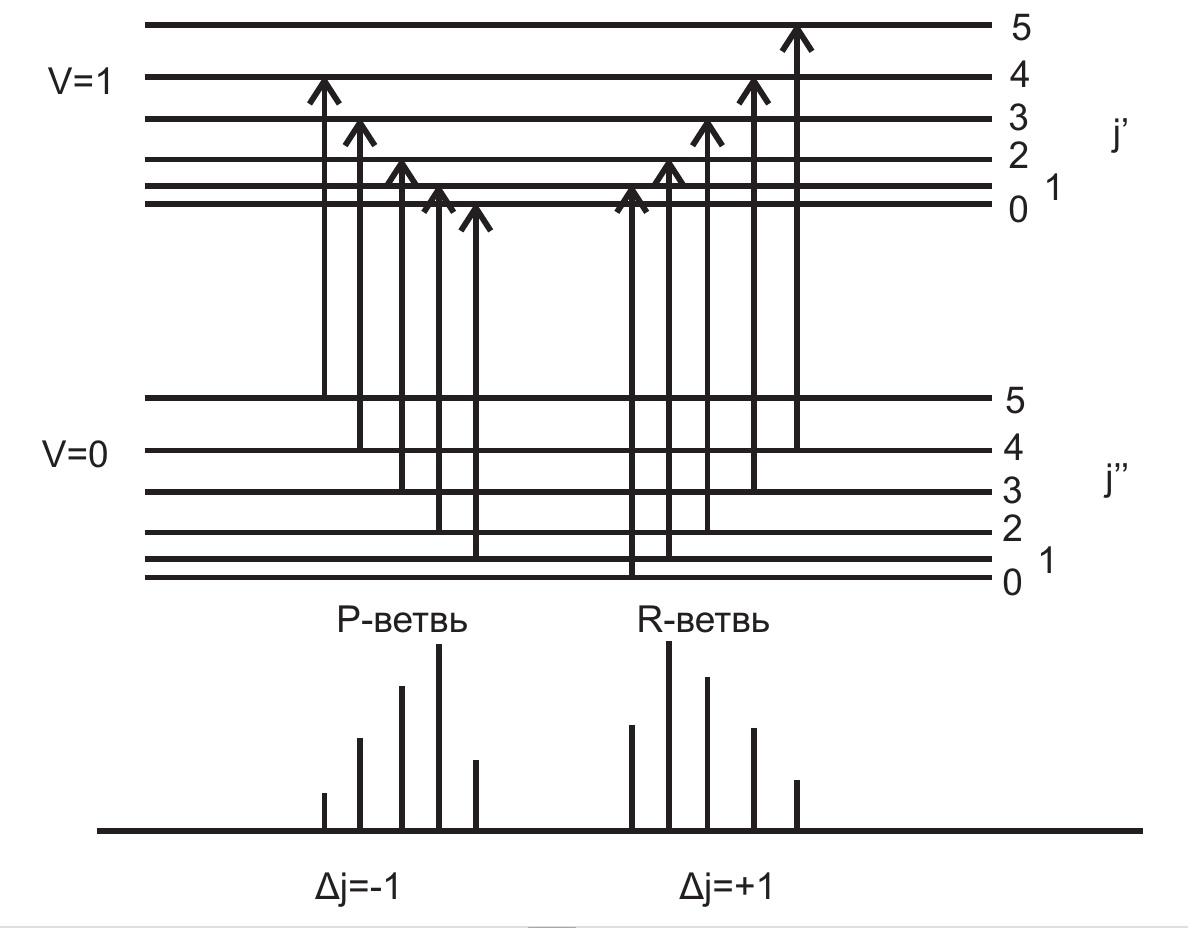
\includegraphics[width=0.8\linewidth]{PR}
	\caption{Формирование $P$ - и $R$-ветвей колебательно-вращательного спектра двухатомной молекулы}
	\label{PR:fig}
\end{figure}

Интенсивность линий в спектре определяется заселенностью энергетических уровней, которая определяется распределением Больцмана
\begin{equation}
n_i = n_0\cfrac{g_i}{g_0}\,\exp{\left(-\cfrac{\Delta E}{kT}\right)}
\end{equation}

Рассмотрение различных вариантов перехода, получаем следующие выражение для волновых чисел
\begin{equation}
\nu_{P, R} = \omega_e(1-2\chi_e)+(B_1+B_0)m+(B_1-B_0)m^2, m = \pm 1, \pm2, \dots
\end{equation}
Так как $B_1 < B_0$, последний член, независимо от знака
$m$, всегда отрицателен, и его влияние на спектр состоит в том, что
с ростом $m$ вращательные линии R-ветви все более сближаются, а
линии P-ветви ($m$ отрицательно) отдаляются друг от друга. Обычно
$B_1$ и $B_0$ различаются незначительно и указанный эффект заметен лишь
для высоких значений $m$.

\subsection{Принципы фурье-спектроскопии}
В её основе принципиальной схемы прибора лежит интерферометр
(здесь --- интерферометр Майкельсона как наиболее распространенный среди используемых во FTIR--спектроскопии). При монохроматическом освещении входного отверстия интерферометра и при равномерном перемещении подвижного зеркала со скоростью $v$ приемником излучения, расположенным за выходной диафрагмой интерферометра, будет регистрироваться переменный сигнал $\Phi(x)$, соответствующий прохождению через выходную диафрагму интерферометра максимумов и минимумов интерференционной картины:
\begin{equation}
\Phi(x) \sim B\cos^2(\pi\nu x)=\cfrac{B}{2}\,(1+\cos(2\pi\nu x))
\end{equation}
Здесь $B$ — яркость светового потока на входе в интерферометр, $x$ —
разность хода, равная удвоенной величине перемещения зеркала $L$ и
линейно зависящая от времени (при равномерной скорости движения
зеркала), $\nu$ — частота излучения. Переменная
составляющая зарегистрированного сигнала равна
\begin{equation}
\Phi(x)=\Phi_0\cos(2\pi\nu x)=\Phi_0\cos(2\pi f t)
\end{equation}
где $f = v\nu = v/\lambda$ — частота модуляции. Таким образом, при монохроматическом освещении входной щели интерферометра приемник
излучения регистрирует синусоидальный сигнал, интенсивность которого пропорциональна интенсивности сигнала на входе интерферометра, а частота зависит от скорости передвижения зеркала и от длины
волны излучения. Например, для зеленой линии ртути ($\lambda = 546$ нм)
при скорости передвижения зеркала $v = 10^{-3}$ мм/с, частота модуляции равна 1.83 Гц. Такой тип модуляции сигнала получил название интерференционной модуляции. Если входное отверстие интерферометра
освещено излучением, имеющим в составе несколько монохроматических компонент, приемником регистрируется суммарный сигнал всех
компонент. Если входное отверстие интерферометра освещено излучением с непрерывным спектром, занимающим область частот от $\nu_1$ до
$\nu_2$, то сигнал, регистрируемый приемником, имеет вид
\begin{equation}
\Phi(x)\sim\int_{\nu_1}^{\nu_2}B_{\nu}(\nu)\cos(2\pi\nu x)d\nu
\end{equation}
где $B_{\nu}$ — спектральная яркость. Данное выражение является фурьепреобразованием функции $B_{\nu}$. Спектральная яркость излучения (то есть фактически спектр излучения) восстанавливается с помощью обратного преобразования Фурье зарегистрированного сигнала:
\begin{equation}
B_{\nu} = 2\int_{0}^{2L}\Phi(x)cos(2\pi\nu x)
\end{equation}
Однако в реальных приборах максимальная разность хода ограничена величиной перемещения зеркала $L$ и меняется в пределах от 0 до
$2L$. При этом вместо первоначальной монохроматической линии
восстановленный спектр имеет линию конечной ширины $a(\nu)$. Это
спектральное распределение, как и в случае щелевых спектральных
приборов, принято называть аппаратной функцией. Выражение
можно представить в вид
\begin{equation}
B_{\nu} = 2\int_{-\infty}^{+\infty}\Phi(x)D(x)cos(2\pi\nu x),  
\end{equation}
где $D(x)$ --- прямоугольная функция.

Аппаратную функцию можно улучшить, если вместо прямоугольной
функции взять функцию другого вида. Данный прием называется
аподизацией.
\begin{figure}[h!]
	\centering
	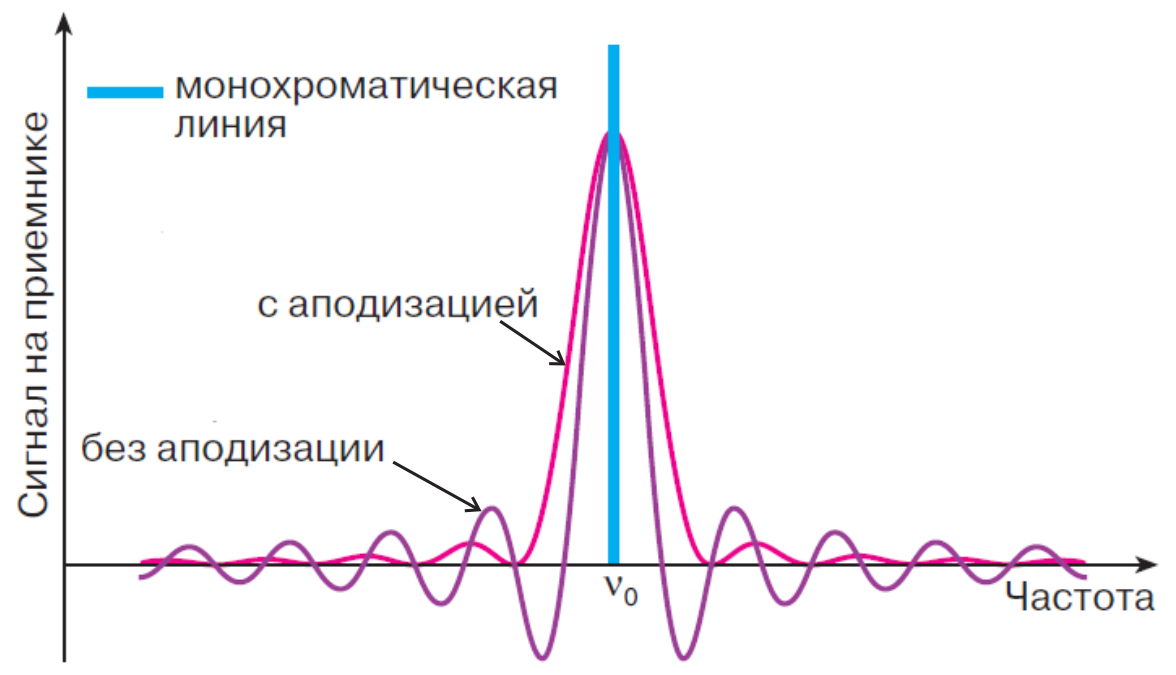
\includegraphics[width=0.7\linewidth]{apotis_graph}
	\caption{Аппаратная функция фурье-спектрометра. Аппаратная функция
		улучшается, если использовать аподизирующую функцию $D(x)$}
	\label{PR:apotis_pg}
\end{figure}
\subsubsection{Преимущества фурье-спектроскопии}
Преимущества фурье-спектроскопии перед другими спектроскопическими методами, использующими разложение в спектр, определяются прежде всего энергетическими выигрышами, получившими название выигрыша Жакино и выигрыша Фелжетта.

Первый обусловлен тем, что у фурье-спектрометров входное отверстие гораздо больше, чем у дисперсионных приборов, свет в которые
попадает через узкую входную щель. Этот выигрыш  может доходить до сотен раз.

Второй выигрыш (Фелжетта) связан с тем, что в обычных спектрометрах регистрируется каждый спектральный интервал поочередно, в то время как в фурье-спектрометрах время регистрации каждого
спектрального интервала равно времени регистрации всего спектра.
Выигрыш Фелжетта пропорционален $M$, где $M$ – число разрешаемых
интервалов в зарегистрированном спектре.  Оба фактора вместе могут
давать выигрыш в величине регистрируемой энергии в четыре порядка.
Одним из преимуществ метода является независимость спектрального разрешения от размеров оптических элементов. Трудно ожидать,
что размеры дифракционных решеток или тем более призм будут больше 50 см. Таким образом, естественным пределом разрешения приборов, использующих пространственную дисперсию, является величина
$0.02$ см$^{-1}$. В то же время уже сейчас налажен серийный промышленный выпуск фурье-спектрометров с разрешением до $0.002$ см$^{-1}$.

Поскольку фурье-спектрометры не требуют очень узких входных и
выходных щелей, требования к созданию оптических схем без аберраций при их конструкции сильно снижаются. По этой причине становится возможным создание оптических схем с большим отношением
диаметра объектива к его фокусу (относительным отверстием), обычно 1:3, что делает такие приборы более компактными при одинаковой
светосиле по сравнению со щелевыми. Такое преимущество оказывается тем более важным, что для обеспечения максимально широкого
спектрального диапазона в спектральных приборах обычно применяется зеркальная оптика, для которой безаберрационные схемы создавать
труднее, чем при использовании линз.


